\documentclass[journal,12pt,twocolumn]{IEEEtran}
%
\usepackage{setspace}
\usepackage{gensymb}
\usepackage{xcolor}
\usepackage{caption}
%\usepackage{subcaption}
%\doublespacing
\singlespacing
\usepackage{multicol}
%\usepackage{eenrc}
\usepackage{iithtlc}
%\usepackage{graphicx}
%\usepackage{amssymb}
%\usepackage{relsize}
\usepackage[cmex10]{amsmath}
\usepackage{mathtools}
%\usepackage{amsthm}
%\interdisplaylinepenalty=2500
%\savesymbol{iint}
%\usepackage{txfonts}
%\restoresymbol{TXF}{iint}
%\usepackage{wasysym}
\usepackage{amsthm}
\usepackage{mathrsfs}
\usepackage{txfonts}
\usepackage{stfloats}
\usepackage{cite}
\usepackage{cases}
\usepackage{subfig}
%\usepackage{xtab}
\usepackage{longtable}
\usepackage{multirow}
%\usepackage{algorithm}
%\usepackage{algpseudocode}
\usepackage{enumitem}
\usepackage{mathtools}
%\usepackage{stmaryrd}
\usepackage{graphicx}
\usepackage{listings}
    \usepackage[latin1]{inputenc}                                 %%
    \usepackage{color}                                            %%
    \usepackage{array}                                            %%
    \usepackage{longtable}                                        %%
    \usepackage{calc}                                             %%
    \usepackage{multirow}                                         %%
    \usepackage{hhline}                                           %%
    \usepackage{ifthen}                                           %%
  %optionally (for landscape tables embedded in another document): %%
    \usepackage{lscape}     
\usepackage{url}
\def\UrlBreaks{\do\/\do-}

%\usepackage{wasysym}
%\newcounter{MYtempeqncnt}
\DeclareMathOperator*{\Res}{Res}
%\renewcommand{\baselinestretch}{2}
\renewcommand\thesection{\arabic{section}}
\renewcommand\thesubsection{\thesection.\arabic{subsection}}
\renewcommand\thesubsubsection{\thesubsection.\arabic{subsubsection}}

\renewcommand\thesectiondis{\arabic{section}}
\renewcommand\thesubsectiondis{\thesectiondis.\arabic{subsection}}
\renewcommand\thesubsubsectiondis{\thesubsectiondis.\arabic{subsubsection}}

% correct bad hyphenation here
\hyphenation{op-tical net-works semi-conduc-tor}

\def\inputGnumericTable{}  

\lstset{
language=python,
frame=single, 
breaklines=true
}

\begin{document}
%

\theoremstyle{definition}

\newtheorem{theorem}{Theorem}[section]
\newtheorem{problem}{Problem}
\newtheorem{proposition}{Proposition}[section]
\newtheorem{lemma}{Lemma}[section]
\newtheorem{corollary}[theorem]{Corollary}
\newtheorem{example}{Example}[section]
\newtheorem{definition}{Definition}[section]
%\newtheorem{algorithm}{Algorithm}[section]
%\newtheorem{cor}{Corollary}
\newcommand{\BEQA}{\begin{eqnarray}}
\newcommand{\EEQA}{\end{eqnarray}}
\newcommand{\define}{\stackrel{\triangle}{=}}

\bibliographystyle{IEEEtran}
%\bibliographystyle{ieeetr}



\providecommand{\pr}[1]{\ensuremath{\Pr\left(#1\right)}}
\providecommand{\qfunc}[1]{\ensuremath{Q\left(#1\right)}}
\providecommand{\sbrak}[1]{\ensuremath{{}\left[#1\right]}}
\providecommand{\lsbrak}[1]{\ensuremath{{}\left[#1\right.}}
\providecommand{\rsbrak}[1]{\ensuremath{{}\left.#1\right]}}
\providecommand{\brak}[1]{\ensuremath{\left(#1\right)}}
\providecommand{\lbrak}[1]{\ensuremath{\left(#1\right.}}
\providecommand{\rbrak}[1]{\ensuremath{\left.#1\right)}}
\providecommand{\cbrak}[1]{\ensuremath{\left\{#1\right\}}}
\providecommand{\lcbrak}[1]{\ensuremath{\left\{#1\right.}}
\providecommand{\rcbrak}[1]{\ensuremath{\left.#1\right\}}}
\theoremstyle{remark}
\newtheorem{rem}{Remark}
\newcommand{\sgn}{\mathop{\mathrm{sgn}}}
\providecommand{\abs}[1]{\left\vert#1\right\vert}
\providecommand{\res}[1]{\Res\displaylimits_{#1}} 
\providecommand{\norm}[1]{\lVert#1\rVert}
\providecommand{\mtx}[1]{\mathbf{#1}}
\providecommand{\mean}[1]{E\left[ #1 \right]}
\providecommand{\fourier}{\overset{\mathcal{F}}{ \rightleftharpoons}}
%\providecommand{\hilbert}{\overset{\mathcal{H}}{ \rightleftharpoons}}
\providecommand{\system}{\overset{\mathcal{H}}{ \longleftrightarrow}}
\providecommand{\gauss}[2]{\mathcal{N}\ensuremath{\left(#1,#2\right)}}
	%\newcommand{\solution}[2]{\textbf{Solution:}{#1}}
\newcommand{\solution}{\noindent \textbf{Solution: }}
\providecommand{\dec}[2]{\ensuremath{\overset{#1}{\underset{#2}{\gtrless}}}}
%\numberwithin{equation}{section}
%\numberwithin{problem}{section}

\def\putbox#1#2#3{\makebox[0in][l]{\makebox[#1][l]{}\raisebox{\baselineskip}[0in][0in]{\raisebox{#2}[0in][0in]{#3}}}}
     \def\rightbox#1{\makebox[0in][r]{#1}}
     \def\centbox#1{\makebox[0in]{#1}}
     \def\topbox#1{\raisebox{-\baselineskip}[0in][0in]{#1}}
     \def\midbox#1{\raisebox{-0.5\baselineskip}[0in][0in]{#1}}


% paper title
% can use linebreaks \\ within to get better formatting as desired

%\title{FM Signal Transmission Using Pi}
 
\title{
\logo{
Digital System Design using Arduino
}
} 
 
%
%
% author names and IEEE memberships
% note positions of commas and nonbreaking spaces ( ~ ) LaTeX will not break
% a structure at a ~ so this keeps an author's name from being broken across
% two lines.
% use \thanks{} to gain access to the first footnote area
% a separate \thanks must be used for each paragraph as LaTeX2e's \thanks
% was not built to handle multiple paragraphs
%

%\author{Y Aditya, A Rathnakar and G V V Sharma$^{*}$% <-this % stops a space
\author{K Prasanna Kumar %<-this  stops a space

\thanks{The author is a project associate with the National Resource Centre, IIT, Hyderabad
502285 India e-mail: kk.prassu924@gmail.com. 
}}



% make the title area
\maketitle


\tableofcontents

\bigskip
\begin{abstract}
This module explains how do design a digital logic circuit using Arduino.
\end{abstract}
\section{Basic Gates}
%\problem Fundamental gates
\subsection{Fundamental gates}
\begin{table}[h!]
\centering
\begin{tabular}{|cc|c|c|c|}
\hline
A	&	B	&	$\overline{A}$	&	AB	&	A + B	\\ \hline
0	&	0	&	1	&	0	&	0 \\ \hline
0	&	1	&	1	&	0	&	1 \\\hline
1	&	0	&	0	&	0	&	1 \\\hline
1	&	1	&	0	&	1	&	1 \\\hline	

\end{tabular}
\end{table}
\lstinputlisting{exp1/exp1.ino}
%\problem Universal gates
\subsection{Universal Gates}
\begin{table}[h!]
\centering
\begin{tabular}{|cc|c|c|}
\hline
A	&	B	&	    	$\overline{AB}$	&	$\overline{A + B}$	\\ \hline
0	&	0	&		    1    	&	1 \\ \hline
0	&	1	&			1		&	0 \\\hline
1	&	0	&			1		&	0 \\\hline
1	&	1	&			0		&	0 \\\hline	

\end{tabular}
\end{table}
\lstinputlisting{exp2/exp2.ino}
\subsection{Exclusive OR and NOR gates}
%\problem Exclusive OR and NOR gates
\begin{table}[h!]
\centering
\begin{tabular}{|cc|c|c|}
\hline
A	&	B	&	     $A\overline{B} + \overline{A}B$	&	$\overline{A\overline{B} + \overline{A}B}$	\\ \hline
0	&	0	&		    0    	&	1 \\ \hline
0	&	1	&			1		&	0 \\\hline
1	&	0	&			1		&	0 \\\hline
1	&	1	&			0		&	1 \\\hline	

\end{tabular}
\end{table}
\lstinputlisting{exp3/exp3.ino}

\section{Combination Logic Circuits}
\subsection{Adder}
\problem Half adder

\vspace{0.5cm}
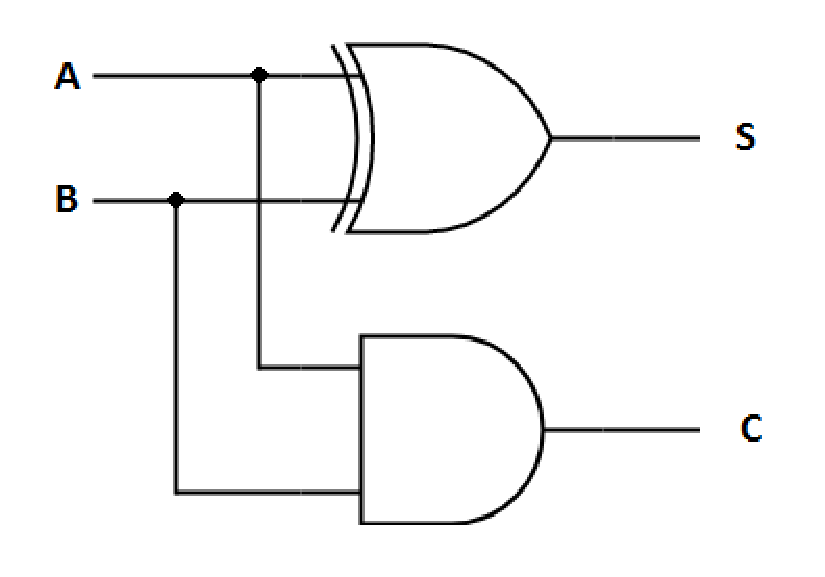
\includegraphics[scale=0.32]{img/Half_Adder}
\begin{table}[h!]
\centering
\begin{tabular}{|cc|c|c|}
\hline
A	&	B	&	   		Sum		&	Carry	\\ \hline
0	&	0	&		    0    	&	0 \\ \hline
0	&	1	&			1		&	0 \\\hline
1	&	0	&			1		&	0 \\\hline
1	&	1	&			0		&	1 \\\hline	

\end{tabular}
\end{table}
\lstinputlisting{exp4/exp4.ino}
\problem Design full adder with basic gates
\problem Design full adder with half adder
\subsection{Subtractor}
\problem Half subtractor

\vspace{0.5cm}
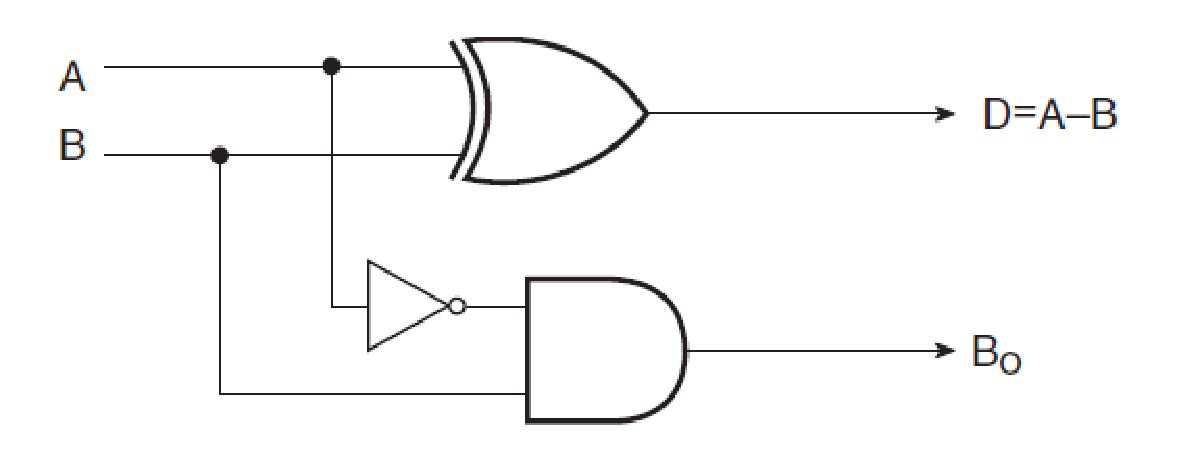
\includegraphics[scale=0.35]{img/half_sub}
\begin{table}[h!]
\centering
\begin{tabular}{|cc|c|c|c|}
\hline
A	&	B	&	NOT A	&	Difference 	&	Borrow	\\ \hline
0	&	0	&	1		&	0	&	0 \\ \hline
0	&	1	&	1		&	0	&	1 \\\hline
1	&	0	&	0		&	0	&	0 \\\hline
1	&	1	&	0		&	1	&	0 \\\hline	

\end{tabular}
\end{table}
\lstinputlisting{exp5/exp5.ino}
\problem Design full subtractor with basic gates
\problem Design full subtractor with half adder
\subsection{Encoder}
\problem 4:2 Encoder

\vspace{0.5cm}
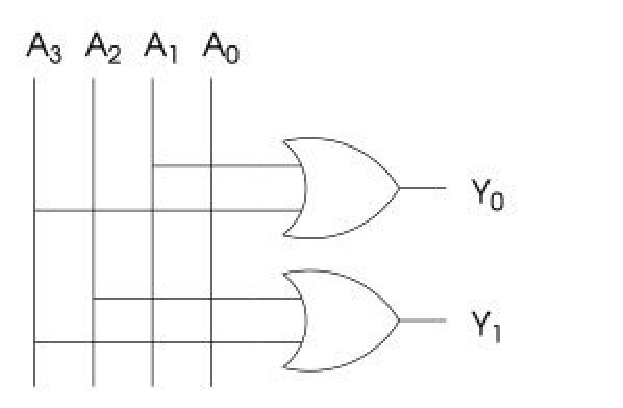
\includegraphics[scale=0.7]{img/42enoder1a}
\begin{table}[h!]
\centering
\begin{tabular}{|cccc|cc|}
\hline
A0	&	A1	&	A2	&	A3	&	Y1	&	Y0 \\\hline
1	&	0	&	0	&	0	&	0	&	0 	\\\hline
0	&	1	&	0	&	0	&	0	&	1	\\\hline
0	&	0	&	1	&	0	&	1	&	0	\\\hline
0	&	0	&	0	&	1	&	1	&	1	\\\hline

\end{tabular}
\end{table}
\lstinputlisting{exp6/exp6.ino}
\problem Design an 8 bit and 16 bit Encoder
\subsection{Decoder}
\problem 2:4 Decoder 

\vspace{0.5cm}
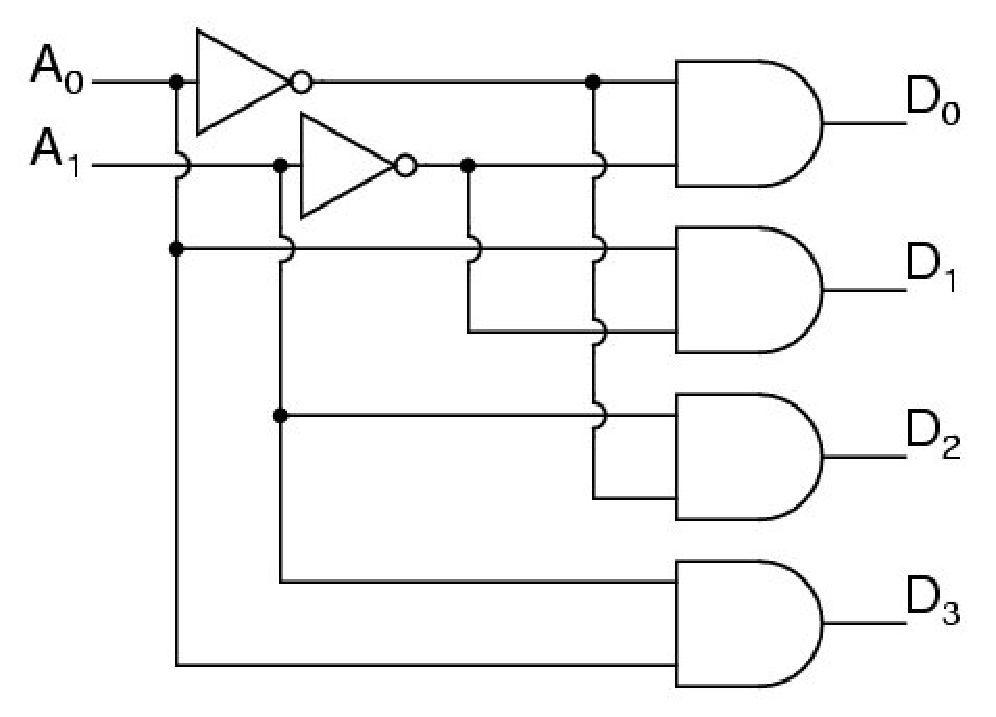
\includegraphics[scale=0.5]{img/24decoder}
\begin{table}[h!]
\centering
\begin{tabular}{|cc|cccc|}
\hline
A1	&	A0	&	D0	&	D1	&	D2	&	D3	 \\\hline
0	&	0	&	1	&	0	&	0	&	0	 	\\\hline
0	&	1	&	0	&	1	&	0	&	0		\\\hline
1	&	0	&	0	&	0	&	1	&	0		\\\hline
1	&	1	&	0	&	0	&	0	&	1		\\\hline

\end{tabular}
\end{table}
\lstinputlisting{exp7/exp7.ino}
\problem Design an 8 bit and 16 bit Decoder
\subsection{Multiplexer}
\problem 4:1 Multiplexer

\vspace{0.5cm}
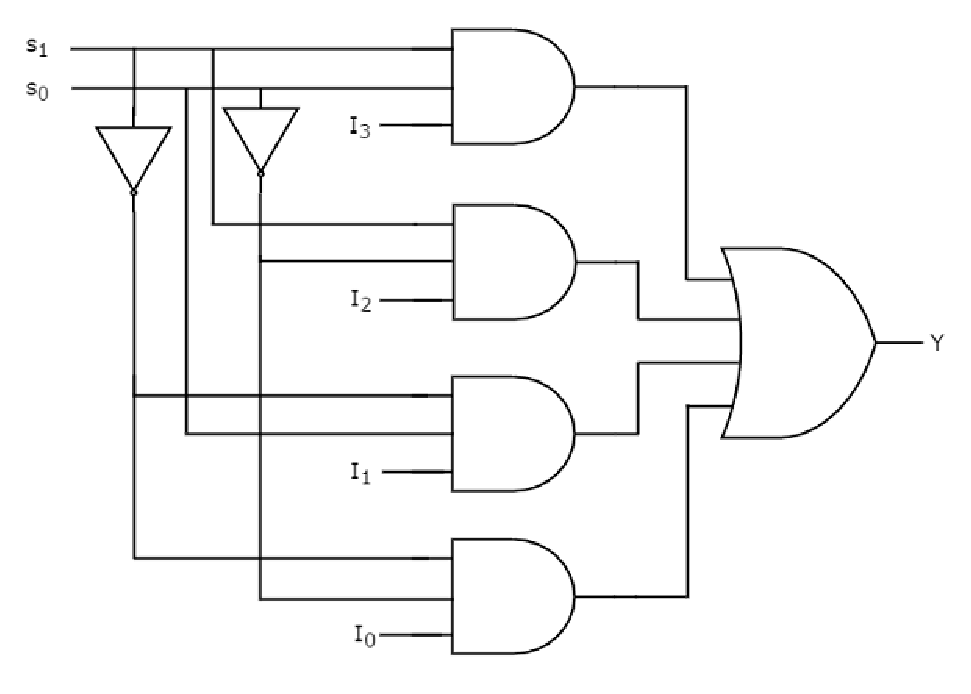
\includegraphics[scale=0.5]{img/41mux}
\begin{table}[h!]
\centering
\begin{tabular}{|cc|c|}
\hline
S0	&	S1	&	Output Y	 \\\hline
0	&	0	&	I0		 	\\\hline
0	&	1	&	I1			\\\hline
1	&	0	&	I2			\\\hline
1	&	1	&	I3			\\\hline

\end{tabular}
\end{table}
\lstinputlisting{exp8/exp8.ino}
\subsection{Demultiplexer}
\problem 1:4 Demultiplexer

\vspace{0.5cm}
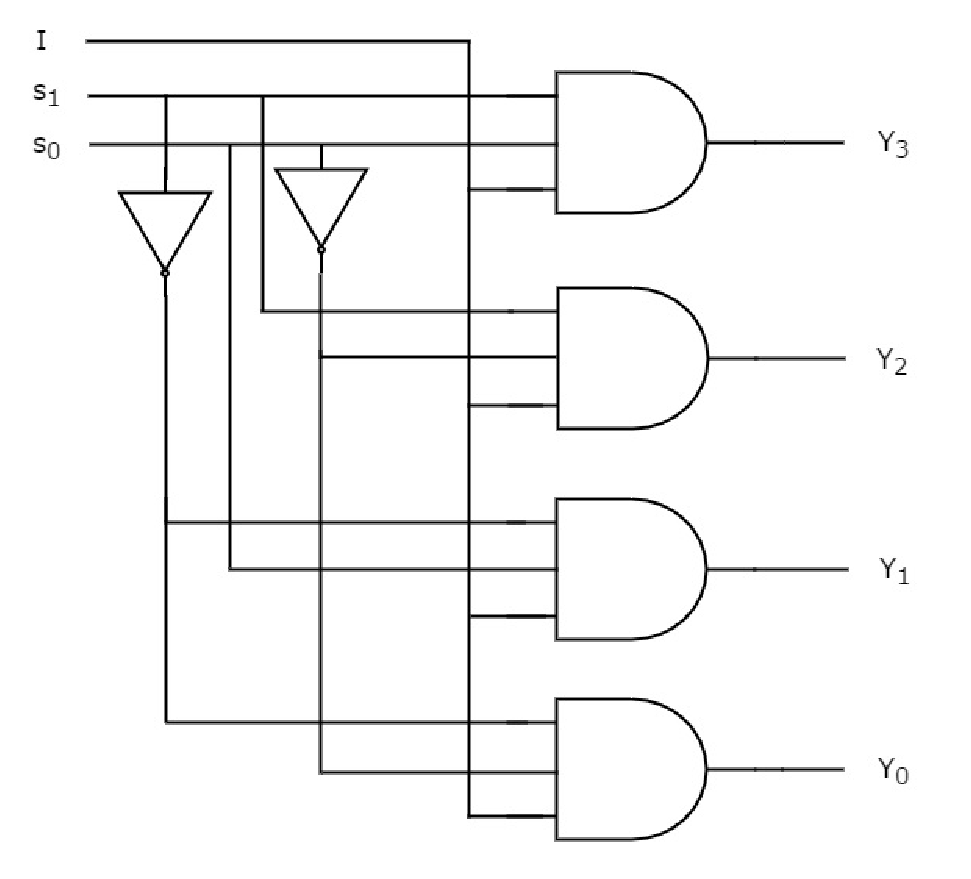
\includegraphics[scale=0.5]{img/14Demux}
\begin{table}[h!]
\centering
\begin{tabular}{|cc|cccc|}
\hline
S0	&	S1	&	D0	&	D1	&	D2	&	D3	 \\\hline
0	&	0	&	I	&	0	&	0	&	0	 	\\\hline
0	&	1	&	0	&	I	&	0	&	0		\\\hline
1	&	0	&	0	&	0	&	I	&	0		\\\hline
1	&	1	&	0	&	0	&	0	&	I		\\\hline

\end{tabular}
\end{table}
\lstinputlisting{exp9/exp9.ino}
\problem Design Mux and De-Mux with 3,4 and 5 input select lines
\subsection{Comparator}
\problem Design 2-bit comparator using Arduino

\vspace{0.5cm}
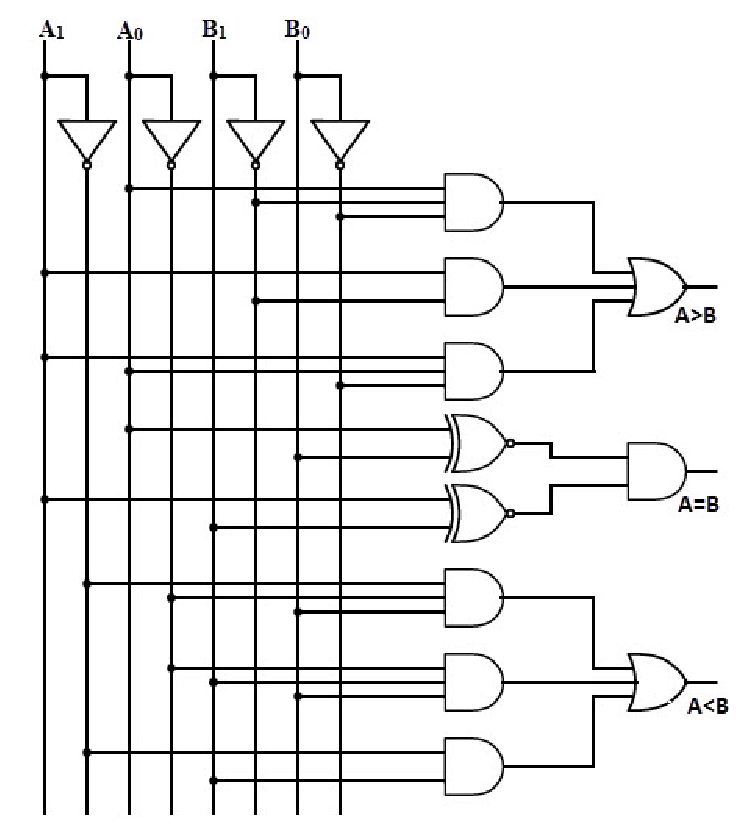
\includegraphics[width = 7cm, height = 7.7cm]{img/2-Bit-Comparator-Logic-Diagram}

using the following truth table to verify the results

\vspace{0.5cm}
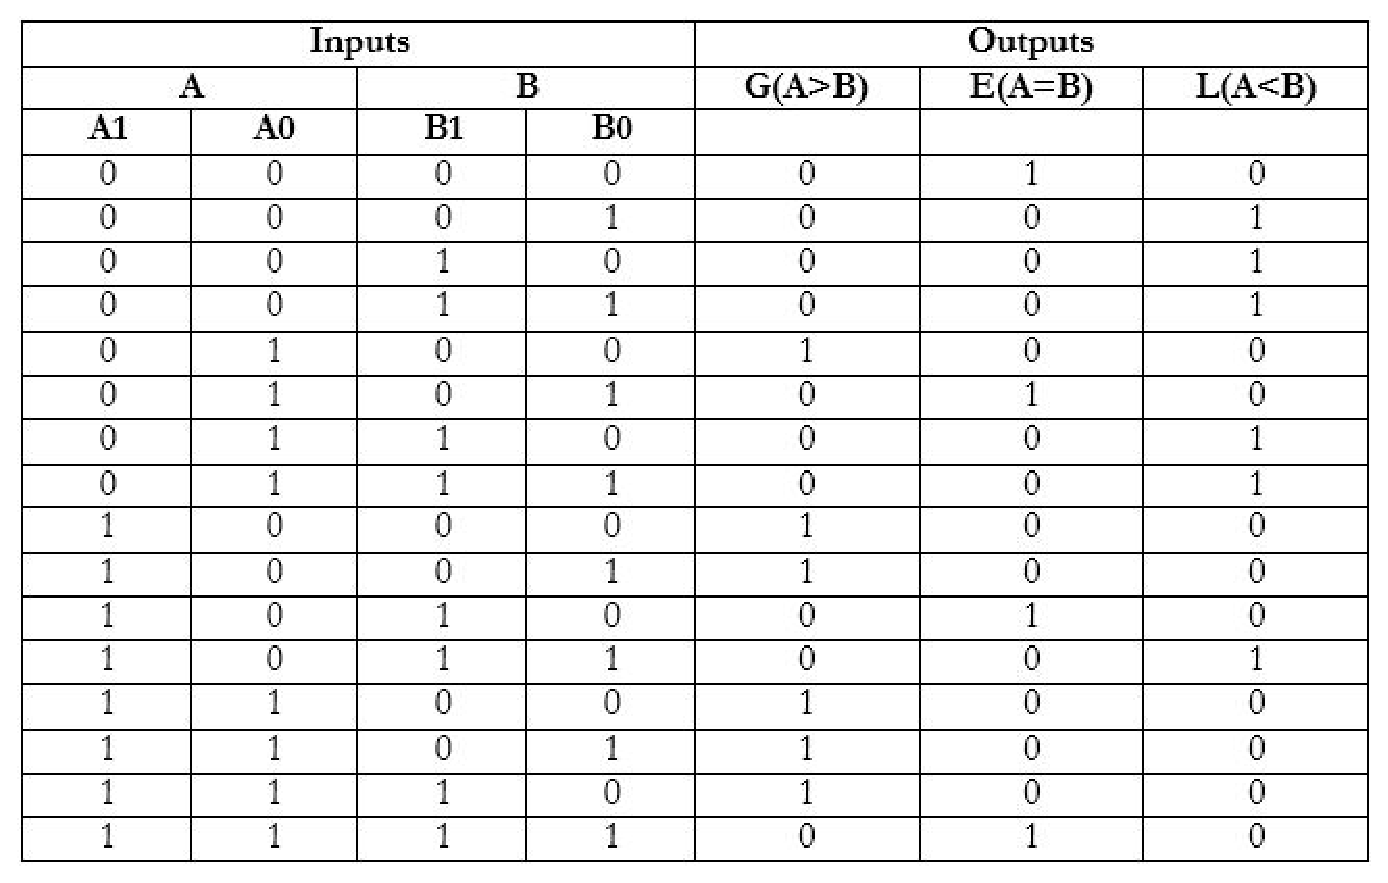
\includegraphics[width = 8.7cm, height = 8cm]{img/2-Bit-Comparator-Truth-Table}
\section{Sequential Logic Circuits}
\subsection{SR Latch}
\problem SR Latch using NAND

\vspace{0.5cm}
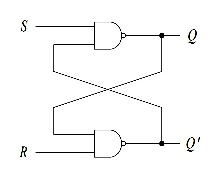
\includegraphics[width = 6cm, height = 4.5cm]{img/SRLatch}
\begin{table}[h!]
\centering
\begin{tabular}{|cc|cc|c|}
\hline
S	&	R	&	$Q_n$	&	$\overline{Q_n}$	& Condition \\\hline
0	&	0	&	 -		&		-		&	Not used		\\\hline
0	&	1	&	1		&		0		&		-	\\\hline
1	&	0	&	0		&		1		&		-	\\\hline
1	&	1	&	-		&		-		&	Memory		\\\hline	
\end{tabular}
\end{table}
\lstinputlisting{SRLatch/SRLatch.ino}
\problem SR Latch using NOR
\subsection{SR Flip Flop}
\problem SR Flip Flop using NAND SR Latch

\vspace{0.5cm}
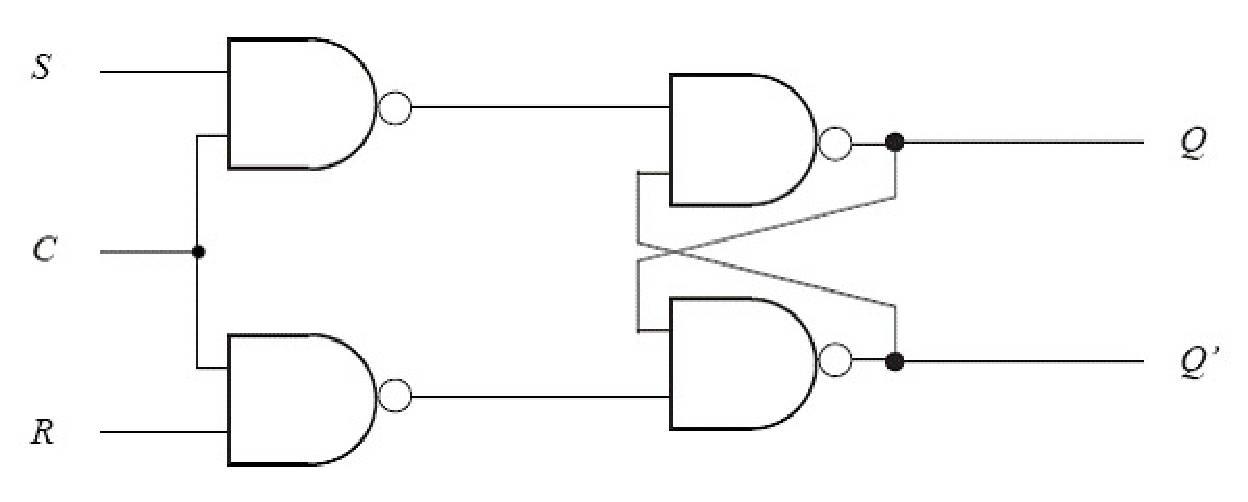
\includegraphics[width = 8cm, height = 3.5cm]{img/SRFlipFlop}
\begin{table}[h!]
\centering
\begin{tabular}{|c|cc|cc|c|}
\hline
CLK	&	S	&	R	&	$Q_n$	&	$\overline{Q_n}$	& Condition \\\hline
1	&	0	&	0	&	 -		&		-		&	Memory		\\\hline
1	&	0	&	1	&	0		&		1		&		-	\\\hline
1	&	1	&	0	&	1		&		0		&		-	\\\hline
1	&	1	&	1	&	-		&		-		&	Not Used		\\\hline	
0	&	x	&	x	&	-		&		-		&	Memory		\\\hline
\end{tabular}
\end{table}
\lstinputlisting{SRFlipflop/SRFlipflop.ino}
\problem SR Flip Flop using NOR SR Latch
\subsection{D Flip Flop}
\problem D Flip Flop using NAND SR Latch

\vspace{0.5cm}
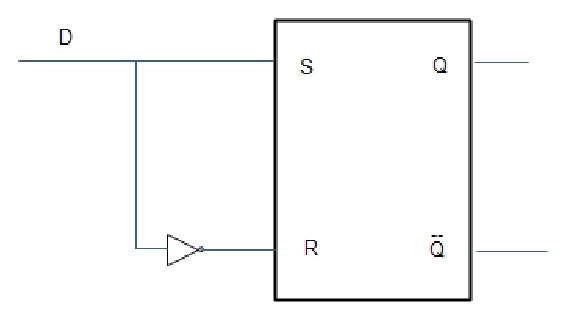
\includegraphics[scale=0.9]{img/D-FF-Circuit}
\begin{table}[h!]
\centering
\begin{tabular}{|c|c|c|}
\hline
CLK	&	D	&	$Q_{n+1}$ \\ \hline
0	&	x	&	$Q_{n}$	\\ \hline
1	&	0	&	D	\\\hline
1	&	1	&	D	\\\hline
\end{tabular}
\end{table}
\lstinputlisting{DFlipflop/DFlipflop.ino}
\problem D Flip Flop using NOR SR Latch
\subsection{JK Flip Flop}
\problem JK Flip Flop using NAND SR Latch

\vspace{0.5cm}
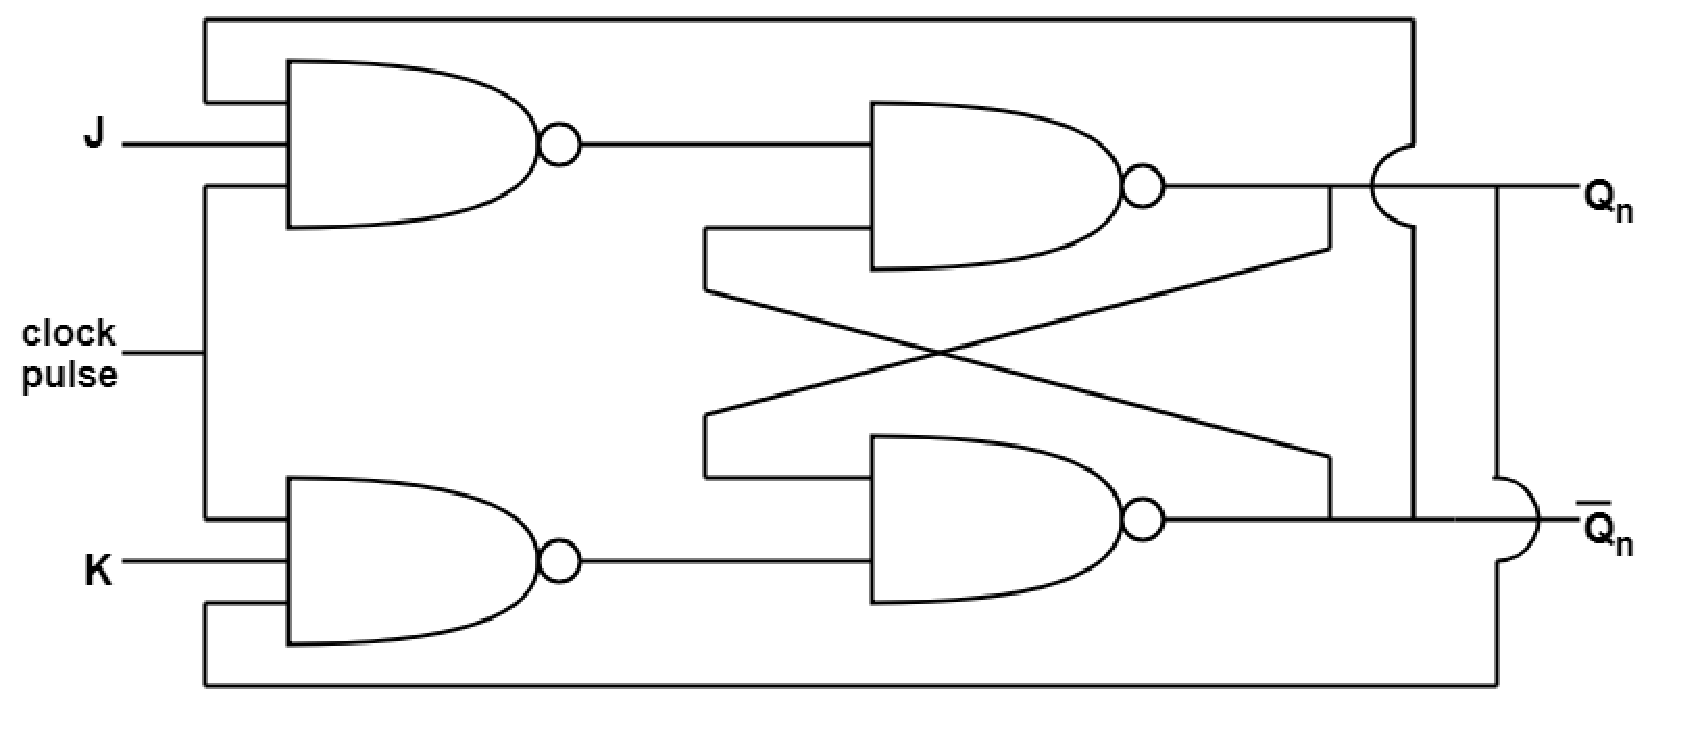
\includegraphics[width = 7cm, height = 5cm]{img/JK-flip-flop}
\begin{table}[h!]
\centering
\begin{tabular}{|c|cc|c|c|}
\hline
CLK	&	J	&	K	&	$Q_{n+1}$		& Condition \\\hline
1	&	0	&	0	&	 $Q_n$		&	Memory		\\\hline
1	&	0	&	1	&	0		&		-	\\\hline
1	&	1	&	0	&	1		&		-	\\\hline
1	&	1	&	1	&	$\overline{Q_n}$&	Toggle		\\\hline	
0	&	x	&	x	&	 $Q_n$		   &	Memory		\\\hline
\end{tabular}
\end{table}
\lstinputlisting{JKFlipflop/JKFlipflop.ino}
\problem JR Flip Flop using NOR SR Latch
\subsection{T Flip Flop}
\problem T Flip Flop using NAND SR Latch

\vspace{0.5cm}
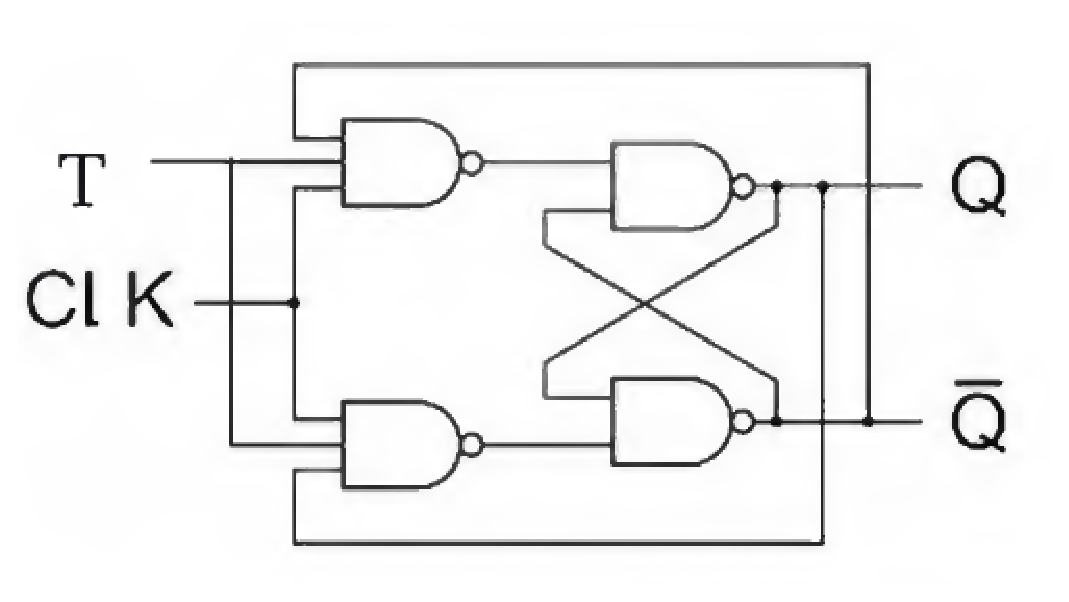
\includegraphics[scale=0.48]{img/T-flip-flop}
\begin{table}[h!]
\centering
\begin{tabular}{|c|c|c|c|}
\hline
CLK	&	T	&	$Q_{n+1}$ & Condition \\ \hline
0	&	x	&	$Q_{n}$	& Memory \\ \hline
1	&	0	&	$Q_{n}$	& Memory \\\hline
1	&	1	&	$\overline{Q_n}$ & Toggle	\\\hline
\end{tabular}
\end{table}
\lstinputlisting{TFlipflop/TFlipflop.ino}
\problem T Flip Flop using NOR SR Latch
\subsection{Counters}
\problem Design 4-Bit up Counter and give the output to 7447 IC, observe the result on SSD
\problem Design 4-Bit  Down Counter and give the output to 7447 IC, observe the result on SSD

%\begin{thebibliography}{00}
%\bibitem{b1} Digital Electronics, 
%Neso Academy, \url{https://www.youtube.com/playlist?list=PLBlnK6fEyqRjMH3mWf6kwqiTbT798eAOm}
%\bibitem{b2} Dr. G.V.V.Sharma, "Digital Design through Arduino", Teaching Learning Centre - IIT Hyderabad
%\end{thebibliography}

\end{document}